\documentclass[tikz, border=12pt]{standalone}
\usepackage{amsmath}
\usetikzlibrary{positioning, arrows.meta}
\begin{document}
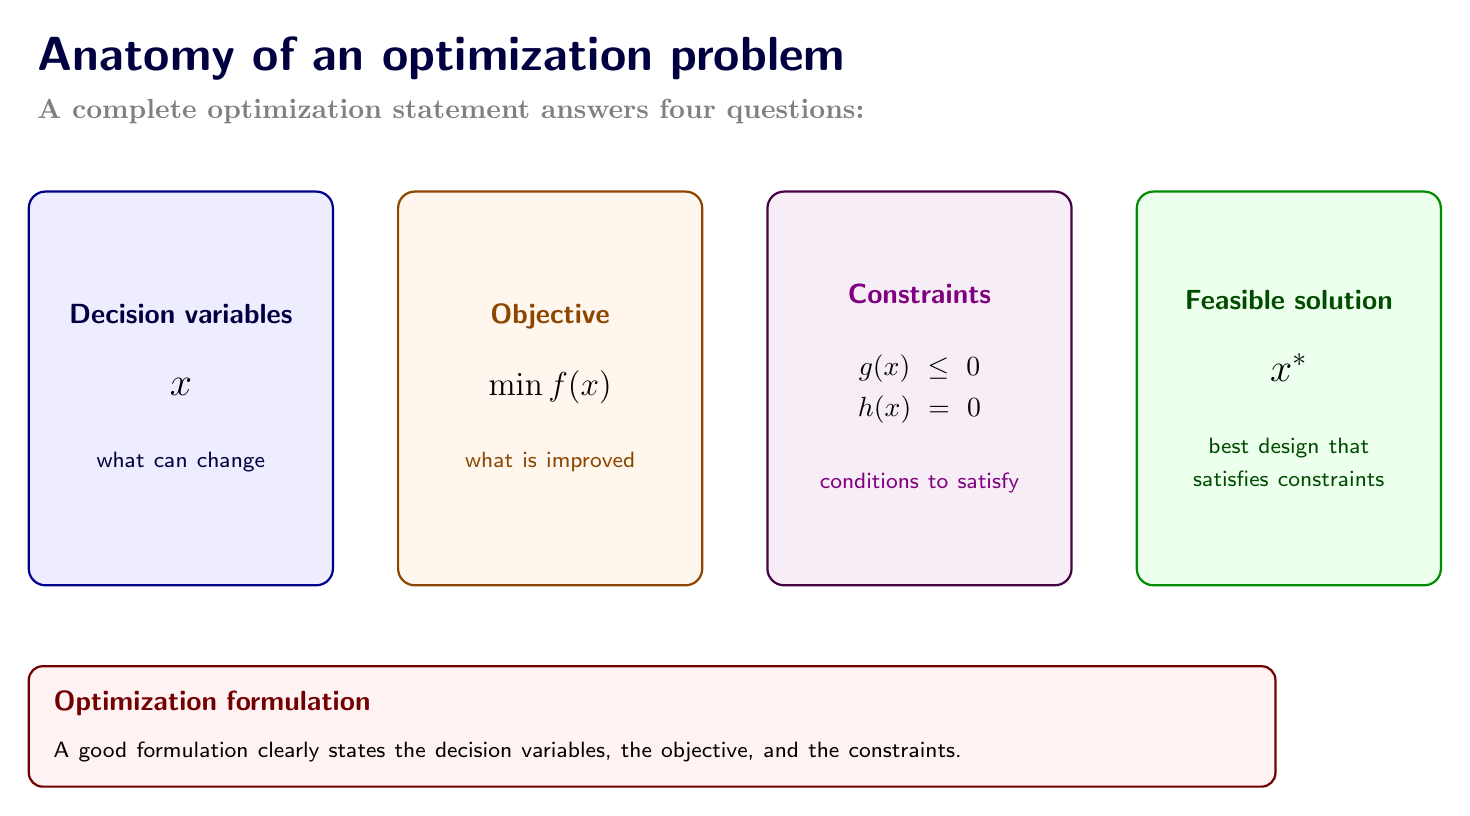
\begin{tikzpicture}[
    font=\sffamily,
    node distance=10mm and 8mm,
    card/.style={rectangle, rounded corners=6pt, draw=#1!55!black, thick,
        fill=#1!7, minimum width=3.6cm, minimum height=5.0cm,
        text width=3.3cm, align=center, inner sep=8pt},
]

\node[font=\sffamily\bfseries\LARGE, text=blue!25!black, anchor=north west] (title) at (0,0)
    {Anatomy of an optimization problem};
\node[below=4mm of title.west, anchor=north west, font=\bfseries, text=gray] (subtitle)
    {A complete optimization statement answers four questions:};

\node[card=blue, below=of subtitle.west, anchor=north west] (dv)
    {\textcolor{blue!25!black}{\bfseries Decision variables}\\[14pt]
     {\Large $x$}\\[14pt]
     \textcolor{blue!25!black}{\footnotesize what can change}};

\node[card=orange, right=of dv] (obj)
    {\textcolor{orange!55!black}{\bfseries Objective}\\[14pt]
     {\large $\min f(x)$}\\[14pt]
     \textcolor{orange!55!black}{\footnotesize what is improved}};

\node[card=violet, right=of obj] (con)
    {\textcolor{violet}{\bfseries Constraints}\\[14pt]
     {$g(x)\le 0$}\\[3pt]
     {$h(x)=0$}\\[14pt]
     \textcolor{violet}{\footnotesize conditions to satisfy}};

\node[card=green, right=of con] (feas)
    {\textcolor{green!30!black}{\bfseries Feasible solution}\\[14pt]
     {\Large $x^{*}$}\\[14pt]
     \textcolor{green!30!black}{\footnotesize best design that satisfies constraints}};

\node[below=10mm of dv.south west, anchor=north west, text width=15.2cm, align=left,
      draw=red!45!black, thick, rounded corners=5pt, fill=red!5, inner sep=9pt]
    {\textcolor{red!45!black}{\bfseries Optimization formulation}\\[5pt]
     \footnotesize A good formulation clearly states the decision variables, the objective, and the constraints.};

\end{tikzpicture}
\end{document}
